\documentclass[10pt,a4paper]{article}
\usepackage[utf8]{inputenc}
\usepackage[a4paper, margin=1.3cm, top=1.4cm, bottom=1.4cm]{geometry}
\usepackage{amsmath,amssymb}
\usepackage{xcolor}
\usepackage[most]{tcolorbox}
\usepackage{booktabs}
\usepackage{colortbl}
\usepackage{fancyhdr}
\usepackage{graphicx}
\usepackage{enumitem}

% Exact colors from previous lecture notes
\definecolor{themeblue}{rgb}{0.1686, 0.3529, 0.5294}   % #2B5A87
\definecolor{lightbg}{rgb}{0.9098, 0.9333, 0.9569}     % #E8EEF4
\definecolor{accentred}{rgb}{0.7843, 0.2706, 0.2275}   % #C8453A

% Header and Footer
\pagestyle{fancy}
\fancyhf{}
\fancyhead[L]{\textcolor{themeblue}{\small Lecture 3 --- Data exploration}}
\fancyhead[R]{\textcolor{themeblue}{\small Deep Learning}}
\renewcommand{\headrulewidth}{0.5pt}
\renewcommand{\headrule}{\hbox to\headwidth{\color{themeblue}\leaders\hrule height \headrulewidth\hfill}}
\fancyfoot[C]{\thepage}

\begin{document}

% =========================================================================
% PAGE 1: Title, Objectives, Notation & Section 1: Quality Criteria
% =========================================================================

% Title Block
\begin{center}
    {\LARGE\bfseries\color{themeblue} Clustering (Unsupervised Classification)}\\[2pt]
    {\small\itshape Deep Learning (S.-A. Berrani, ENSIA 2026--2027)}\\[2pt]
    \textcolor{themeblue}{\rule{\textwidth}{0.6pt}}
\end{center}

\vspace{-7pt}

% Core Idea & Notation Box
\begin{tcolorbox}[
    colframe=themeblue,
    colback=lightbg,
    coltitle=white,
    fonttitle=\bfseries\sffamily,
    title={Objective, Applications \& Notation},
    arc=1.5mm,
    boxrule=0.6pt,
    left=6pt, right=6pt, top=3pt, bottom=3pt
]
\textbf{Objective:} Automatically partition a dataset using a similarity measure / distance.
\begin{itemize}[leftmargin=10pt, itemsep=1pt, topsep=1pt]
    \item \textbf{Input:} A set of $N$ vectors describing $N$ individuals (samples, observations) and algorithm parameters.
    \item \textbf{Output:} $k$ clusters ($+$ noise possibly).
    \item \textbf{Applications:}
    \begin{itemize}[leftmargin=8pt, itemsep=0.5pt]
        \item \textit{Summarize large datasets:} Group similar individuals; study characteristics of the group and the \textbf{average individual (centroid)} rather than studying each of the $N$ individuals.
        \item \textit{Image segmentation:} Pixels (values, position) $\to$ homogeneous region = cluster of similar and connected pixels.
        \item \textit{Others:} Bioinformatics (phylogeny trees), business (customer segments, salary hierarchy), image processing (handwritten character shapes), information retrieval (categorizing search results).
    \end{itemize}
    \item \textbf{4 Steps in Practice:} (1) Description of individuals (feature extraction \& selection) $\to$ (2) Definition of a similarity measure (distance) $\to$ (3) Grouping individuals using feature vectors and distance $\to$ (4) Making use of clusters (interpretation, abstraction).
    \item \textbf{Notation:} $n$ (or $N$) individuals ($v \in \mathbb{R}^d$); $k$ clusters; $n_j$ count in cluster $j$; $g_j = \frac{1}{n_j}\sum_{v \in C_j} v$ (cluster centroid); $g = \frac{1}{n}\sum_{i=1}^n v_i = \sum_{j=1}^k \frac{n_j}{n} g_j$ (global centroid); $d(v_i, g_j)$ distance metric.
\end{itemize}
\end{tcolorbox}

\vspace{2pt}

% Section 1: Quality Criteria
\noindent{\Large\bfseries\color{themeblue} 1. Quality Criteria: Intra vs. Inter Variance (Huygens' Theorem)}\par\vspace{2pt}
We seek a clustering where clusters are: (1) \textbf{Tightened on themselves} ($\operatorname{Var}_{\text{intra}}$ low), and (2) \textbf{Far from each other} ($\operatorname{Var}_{\text{inter}}$ high).

\begin{enumerate}[leftmargin=12pt, itemsep=2pt, topsep=1pt, parsep=0pt]
    \item \textbf{Intra-Cluster Variance (Spread of each cluster):}
    \[
    \operatorname{Var}_{\text{intra}} = \frac{1}{n} \sum_{j=1}^k \sum_{i=1}^{n_j} d^2(v_i, g_j) \qquad \longrightarrow \quad \textbf{Goal: Minimize } \operatorname{Var}_{\text{intra}}
    \]
    Measures internal cohesion. Lower intra-cluster variance indicates tightly clustered points around their centroid.

    \item \textbf{Inter-Cluster Variance (Spacing of clusters from each other / Spread of centroids):}
    \[
    \operatorname{Var}_{\text{inter}} = \sum_{j=1}^k \frac{n_j}{n} d^2(g, g_j) \qquad \longrightarrow \quad \textbf{Goal: Maximize } \operatorname{Var}_{\text{inter}}
    \]
    Measures cluster separation. Higher inter-cluster variance indicates cluster centroids are far apart from each other and the global center.

    \item \textbf{Total Variance and Huygens' Theorem:}
    The total variance is the dispersion of all $n$ individuals around the dataset center $g$:
    $\operatorname{Var}_{\text{total}} = \frac{1}{n} \sum_{i=1}^n d^2(v_i, g)$.
    \begin{tcolorbox}[
        colframe=accentred,
        colback=white,
        arc=1.5mm,
        boxrule=0.5pt,
        left=6pt, right=6pt, top=2.5pt, bottom=2.5pt
    ]
    \textbf{Theorem of Huygens:}
    \[
    \mathbf{\operatorname{Var}_{\text{total}} = \operatorname{Var}_{\text{intra}} + \operatorname{Var}_{\text{inter}} = \text{Constant}}
    \]
    \textbf{Why the two goals are equivalent:} The total variance $\operatorname{Var}_{\text{total}}$ is strictly constant (it depends only on the raw dataset points and global mean $g$, not on the clustering). Since $\operatorname{Var}_{\text{inter}} = \operatorname{Var}_{\text{total}} - \operatorname{Var}_{\text{intra}}$, minimizing $\operatorname{Var}_{\text{intra}}$ automatically and mathematically maximizes $\operatorname{Var}_{\text{inter}}$. \textit{All you have to do is to optimize one of the two criteria.}
    \end{tcolorbox}

    \item \textbf{Mathematical Derivation / Proof:}
    Decompose $(v_i - g) = (v_i - g_j) + (g_j - g)$. Expanding the squared Euclidean norm:
    \[
    \|v_i - g\|^2 = \|(v_i - g_j) + (g_j - g)\|^2 = \|v_i - g_j\|^2 + \|g_j - g\|^2 + 2\langle v_i - g_j, \, g_j - g\rangle
    \]
    Summing over all $n_j$ points in cluster $C_j$, the cross-term vanishes because $\sum_{i=1}^{n_j}(v_i - g_j) = n_j g_j - n_j g_j = \mathbf{0}$:
    \[
    \sum_{i=1}^{n_j} \|v_i - g\|^2 = \sum_{i=1}^{n_j} \|v_i - g_j\|^2 + n_j \|g_j - g\|^2 + 2\langle \mathbf{0}, \, g_j - g\rangle = \sum_{i=1}^{n_j} \|v_i - g_j\|^2 + n_j \|g_j - g\|^2
    \]
    Summing across all $k$ clusters ($j=1, \dots, k$) and dividing by total count $n$:
    \[
    \frac{1}{n}\sum_{i=1}^n d^2(v_i, g) = \frac{1}{n}\sum_{j=1}^k\sum_{i=1}^{n_j} d^2(v_i, g_j) + \sum_{j=1}^k \frac{n_j}{n} d^2(g, g_j) \iff \mathbf{\operatorname{Var}_{\text{total}} = \operatorname{Var}_{\text{intra}} + \operatorname{Var}_{\text{inter}}}
    \]
\end{enumerate}

\clearpage

% =========================================================================
% PAGE 2: Variance Plot + Section 2: Overview + Section 3: K-Means
% =========================================================================

{\centering
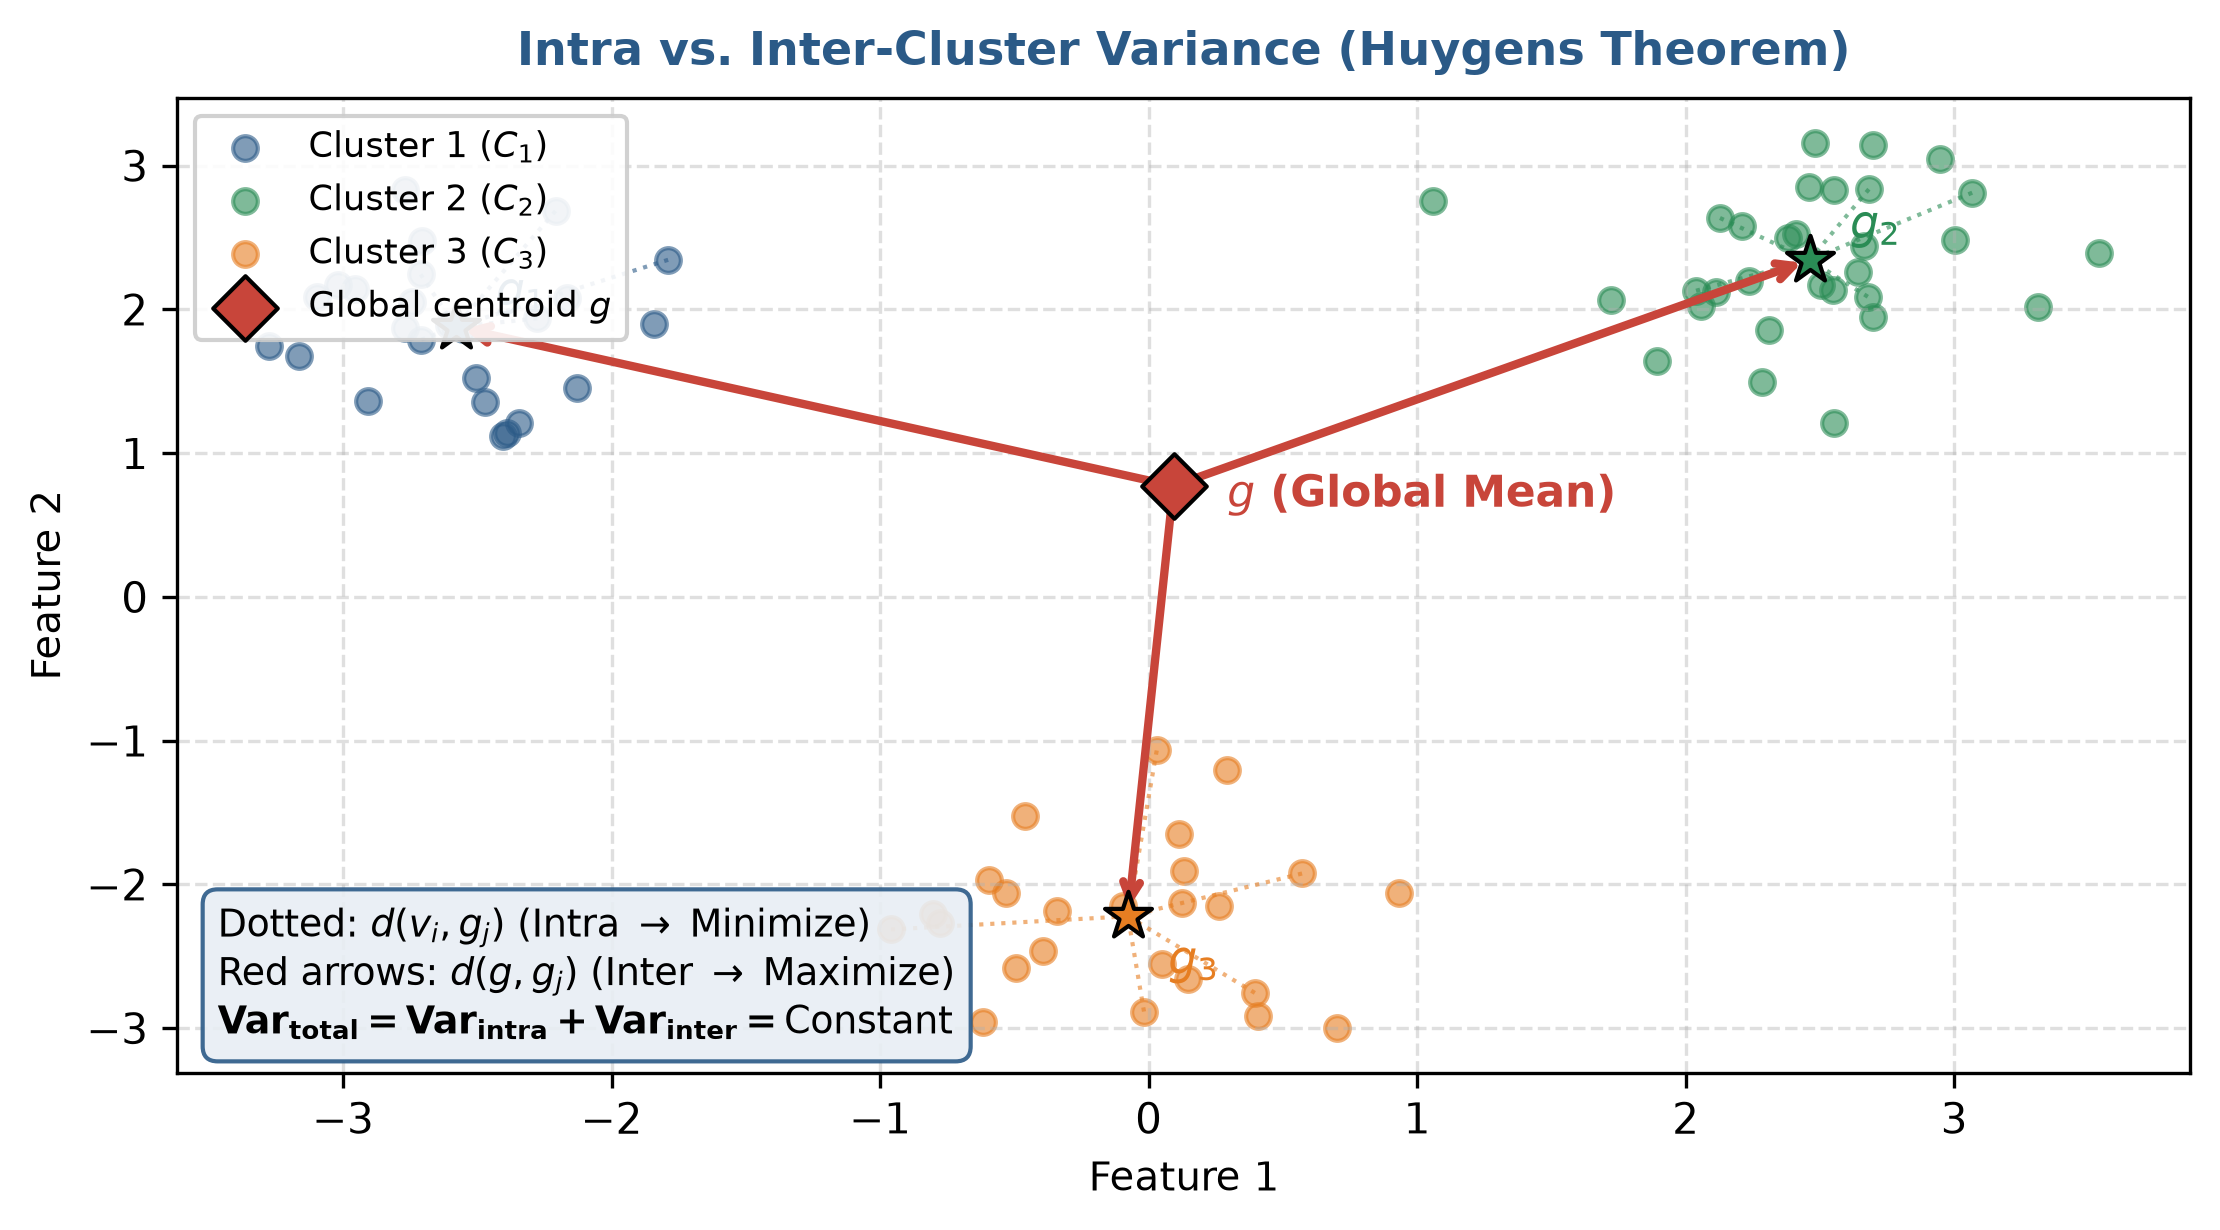
\includegraphics[width=0.55\textwidth]{variance_plot.png}\par
\vspace{1pt}
{\footnotesize\textit{Intra-cluster dispersion $d(v_i, g_j)$ vs. Inter-cluster dispersion $d(g, g_j)$ (Huygens' Theorem).}}\par
}

\vspace{6pt}

% Section 2: Overview of Existing Techniques
\noindent{\Large\bfseries\color{themeblue} 2. Existing Techniques: An Overview}\par\vspace{3pt}
\begin{center}
\small
\begin{tabular}{p{0.22\textwidth}p{0.48\textwidth}p{0.22\textwidth}}
\toprule
\rowcolor{lightbg}
\textbf{Technique Family} & \textbf{Mechanism} & \textbf{Algorithms Listed} \\
\midrule
\textbf{Data partitioning} & Iterative algorithms that refine an initial clustering. & \textbf{K-means}, CLARANS, Kohonen maps \\
\addlinespace[2pt]
\textbf{Hierarchical} & Hierarchical partitioning of the data. & \textbf{Traditional methods}, BIRCH \\
\addlinespace[2pt]
\textbf{Density-based} & Based on density estimation methods (parametric and non-parametric). & DBSCAN, DENCLUE \\
\addlinespace[2pt]
\textbf{Space partitioning} & Space quantization. & STING, Wave Cluster, Opti-Grid \\
\bottomrule
\end{tabular}
\end{center}

\vspace{5pt}

% Section 3: K-Means
\noindent{\Large\bfseries\color{themeblue} 3. K-Means: The Algorithm}\par\vspace{3pt}
K-Means performs \textbf{``clustering around moving centers''}.

\begin{itemize}[leftmargin=12pt, itemsep=1.5pt, topsep=1.5pt]
    \item \textbf{Input:} $N$ individuals; $k$ centers [randomly chosen at the beginning]; $k$ empty clusters.
\end{itemize}

\vspace{1pt}
\noindent\textbf{Algorithm:}
\begin{tcolorbox}[
    colframe=themeblue,
    colback=lightbg,
    arc=1.5mm,
    boxrule=0.5pt,
    left=6pt, right=6pt, top=3pt, bottom=3pt
]
\textbf{Repeat:}
\begin{enumerate}[leftmargin=14pt, itemsep=2pt, topsep=1pt]
    \item \textbf{Distribute} the $N$ individuals over the $k$ clusters using the rule of \textbf{« the nearest center »}:
    \[
    C_j = \big\{ v_i : d(v_i, g_j) \le d(v_i, g_l) \quad \forall l \ne j \big\}
    \]
    \item \textbf{Compute} the new $k$ centers:
    \[
    g_j = \frac{1}{n_j} \sum_{v \in C_j} v
    \]
\end{enumerate}
\textbf{Until} two consecutive ``clusterings'' are identical.
\end{tcolorbox}

\vspace{2pt}
\noindent\textbf{Properties of K-Means:}
\begin{itemize}[leftmargin=12pt, itemsep=2pt, topsep=1pt]
    \item \textbf{Parameters:} The number of clusters $k$ must be specified beforehand.
    \item \textbf{Sensitivity:} Sensitive to initial conditions (non-deterministic).
    \item \textbf{Iterative:} Requires several passes over the dataset.
    \item \textbf{Complexity:} $O(N)$ (linear in the number of individuals).
\end{itemize}

\clearpage

% =========================================================================
% PAGE 3: Section 4: Hierarchical Clustering (4.1 Dendrogram + 4.2 Agglom/Divis)
% =========================================================================

\noindent{\Large\bfseries\color{themeblue} 4. Hierarchical Clustering}\par\vspace{3pt}

\noindent{\large\bfseries\color{themeblue} 4.1 Visual Representation: The Dendrogram \& Cutting Level}\par\vspace{2pt}
\begin{itemize}[leftmargin=12pt, itemsep=1.5pt, topsep=1pt, parsep=0pt]
    \item \textbf{Visual Representation:} Clusters are visually represented in a hierarchical tree called a \textbf{dendrogram}.
    \item \textbf{No Pre-set $k$:} There is no need to pre-specify the number of clusters. Instead, the dendrogram can be cut horizontally at the appropriate level to obtain the desired number of clusters.
    \item \textbf{Summarization \& Interpretation:} Data is easily organized and summarized into a hierarchy using dendrograms; dendrograms make it easy to examine and interpret clusters.
    \item \textbf{Requires a proximity measure} between clusters.
    \item \textbf{Handling Large Datasets:} If we have a very large dataset, the bottom of the dendrogram may be unreadable due to overcrowding of individual leaves $\implies$ \textbf{Solution: Show and focus on the top part of the tree.}
\end{itemize}

\vspace{1pt}
{\centering
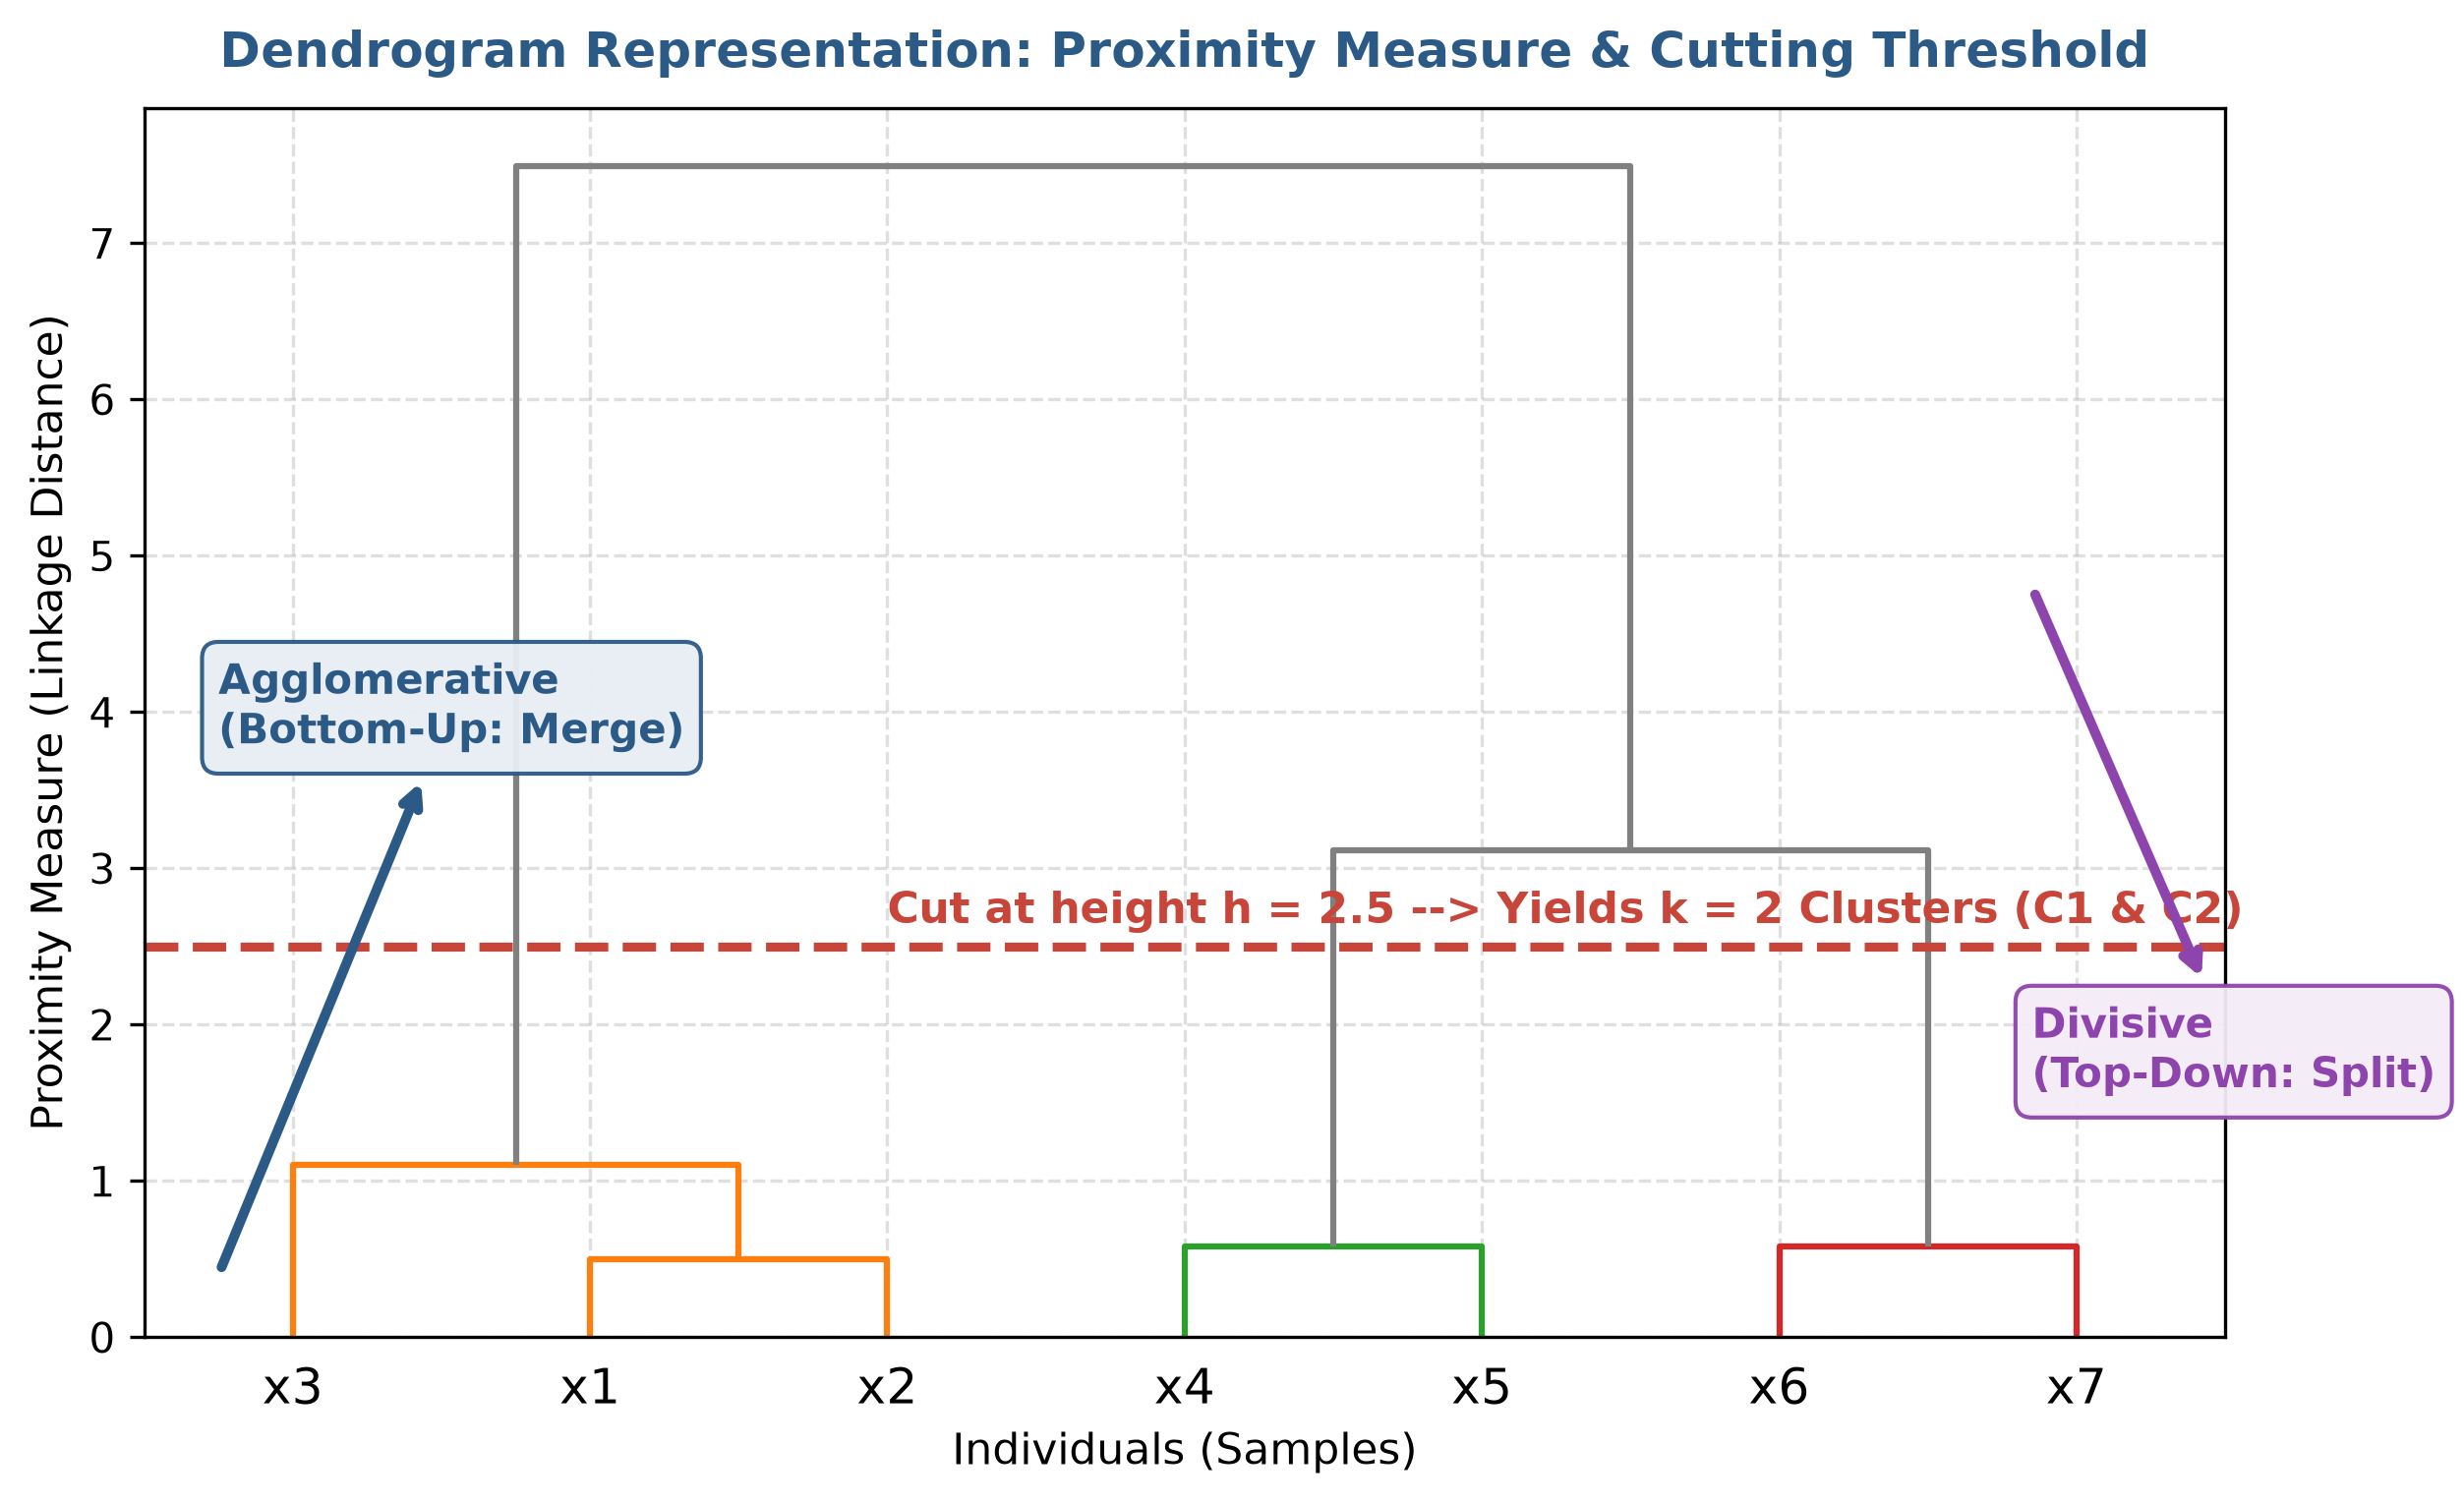
\includegraphics[width=0.68\textwidth]{dendrogram_cut.png}\par
\vspace{1pt}
{\footnotesize\textit{Hierarchical Dendrogram: Horizontal cut at $h = 2.5$ yields $k = 2$ clusters. Higher cuts $\to$ fewer clusters.}}\par
}
\vspace{4pt}

\noindent{\large\bfseries\color{themeblue} 4.2 The Two Main Types: Agglomerative vs. Divisive}\par\vspace{2pt}
\begin{enumerate}[leftmargin=14pt, itemsep=2pt, topsep=1pt, parsep=0pt]
    \item \textbf{Agglomerative (Bottom-Up):} Initially, each object is considered to be its own cluster ($N$ singleton clusters). According to a particular procedure, the clusters are then merged step by step until a single cluster remains containing all elements.
    \item \textbf{Divisive (Top-Down):} Initially, all objects are considered in a single cluster. Then the division process is performed step by step until each object forms a different cluster.
\end{enumerate}

\vspace{1pt}
{\centering
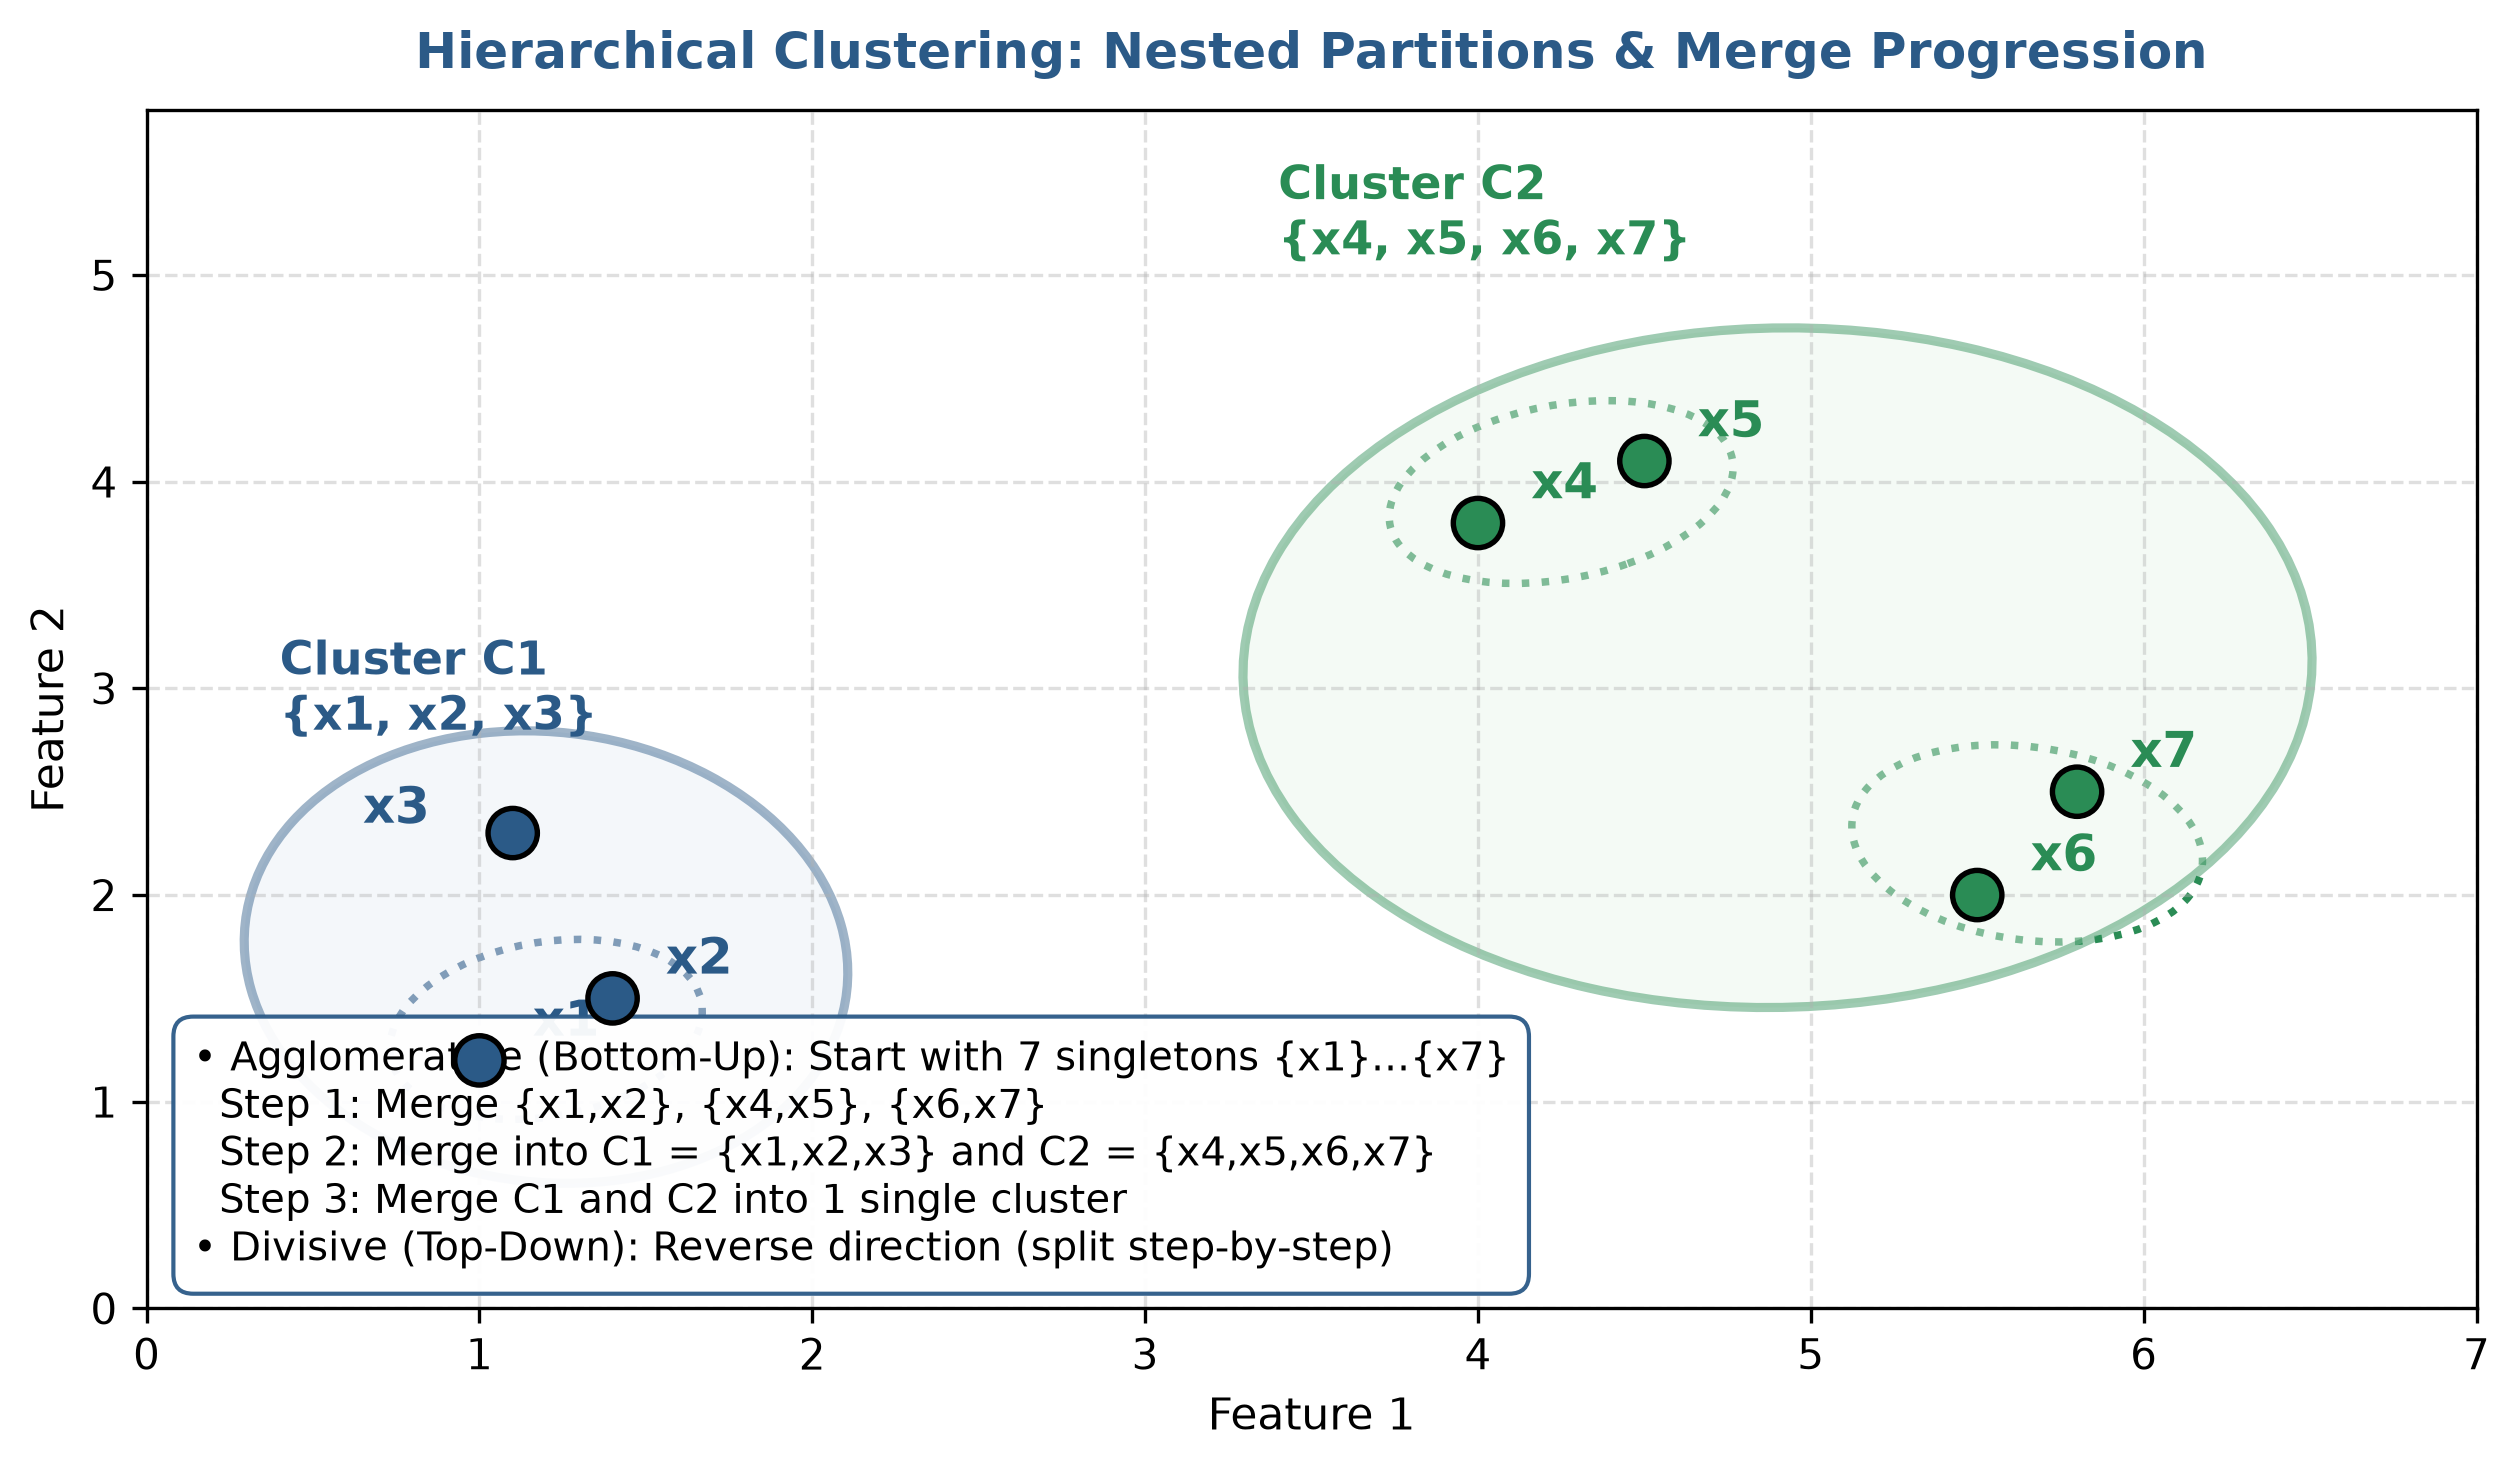
\includegraphics[width=0.68\textwidth]{hierarchical_nested_clusters.png}\par
\vspace{1pt}
{\footnotesize\textit{Nested Partitions \& Merge Progression: Agglomerative (Bottom-Up) vs. Divisive (Top-Down).}}\par
}

\clearpage

% =========================================================================
% PAGE 4: Section 4.3 Linkage Criteria & 4.4 Properties
% =========================================================================

\noindent{\large\bfseries\color{themeblue} 4.3 Proximity / Linkage Criteria Between Clusters}\par\vspace{2pt}
To decide which clusters to merge at each step, a linkage/proximity measure between clusters $C_A$ and $C_B$ is required:

\begin{enumerate}[leftmargin=14pt, itemsep=2pt, topsep=1.5pt, parsep=0pt]
    \item \textbf{Min (Single) Linkage:}
    The distance between 2 clusters is the \textbf{minimum distance} between points in those clusters:
    \[
    d(C_A, C_B) = \min_{x \in C_A, y \in C_B} d(x, y)
    \]

    \item \textbf{Max (Complete) Linkage:}
    The distance between 2 clusters is the \textbf{maximum distance} between points in those clusters:
    \[
    d(C_A, C_B) = \max_{x \in C_A, y \in C_B} d(x, y)
    \]

    \item \textbf{Average Linkage:}
    The distance between 2 clusters is the \textbf{average pairwise distance} among all pairs of points in the clusters:
    \[
    d(C_A, C_B) = \frac{1}{|C_A| |C_B|} \sum_{x \in C_A} \sum_{y \in C_B} d(x, y)
    \]

    \item \textbf{Centroid Linkage:}
    The distance between 2 clusters is the \textbf{distance between their centroids}:
    \[
    d(C_A, C_B) = d(g_A, g_B)
    \]

    \item \textbf{Ward Linkage (Preferred Approach):}
    \begin{tcolorbox}[
        colframe=accentred,
        colback=white,
        arc=1.5mm,
        boxrule=0.5pt,
        left=6pt, right=6pt, top=2.5pt, bottom=2.5pt
    ]
    \textbf{Principle of Ward's Method:}
    \begin{itemize}[leftmargin=10pt, itemsep=1.5pt, topsep=1pt]
        \item The Ward approach \textbf{analyzes the variance of the clusters} rather than measuring distances directly, minimizing the variance between clusters.
        \item It consists of grouping clusters so that the \textbf{increase in inter-cluster variance is maximum}.
        \item This amounts to the same thing according to \textbf{Huygens' theorem}: \textbf{The increase in intra-class inertia is minimum}:
        \[
        \Delta \operatorname{Var}_{\text{intra}}(C_A, C_B) = \frac{n_A n_B}{n_A + n_B} d^2(g_A, g_B)
        \]
        \item \textbf{Ward's method is preferred more than others in clustering.}
    \end{itemize}
    \end{tcolorbox}
\end{enumerate}

\vspace{1pt}
{\centering
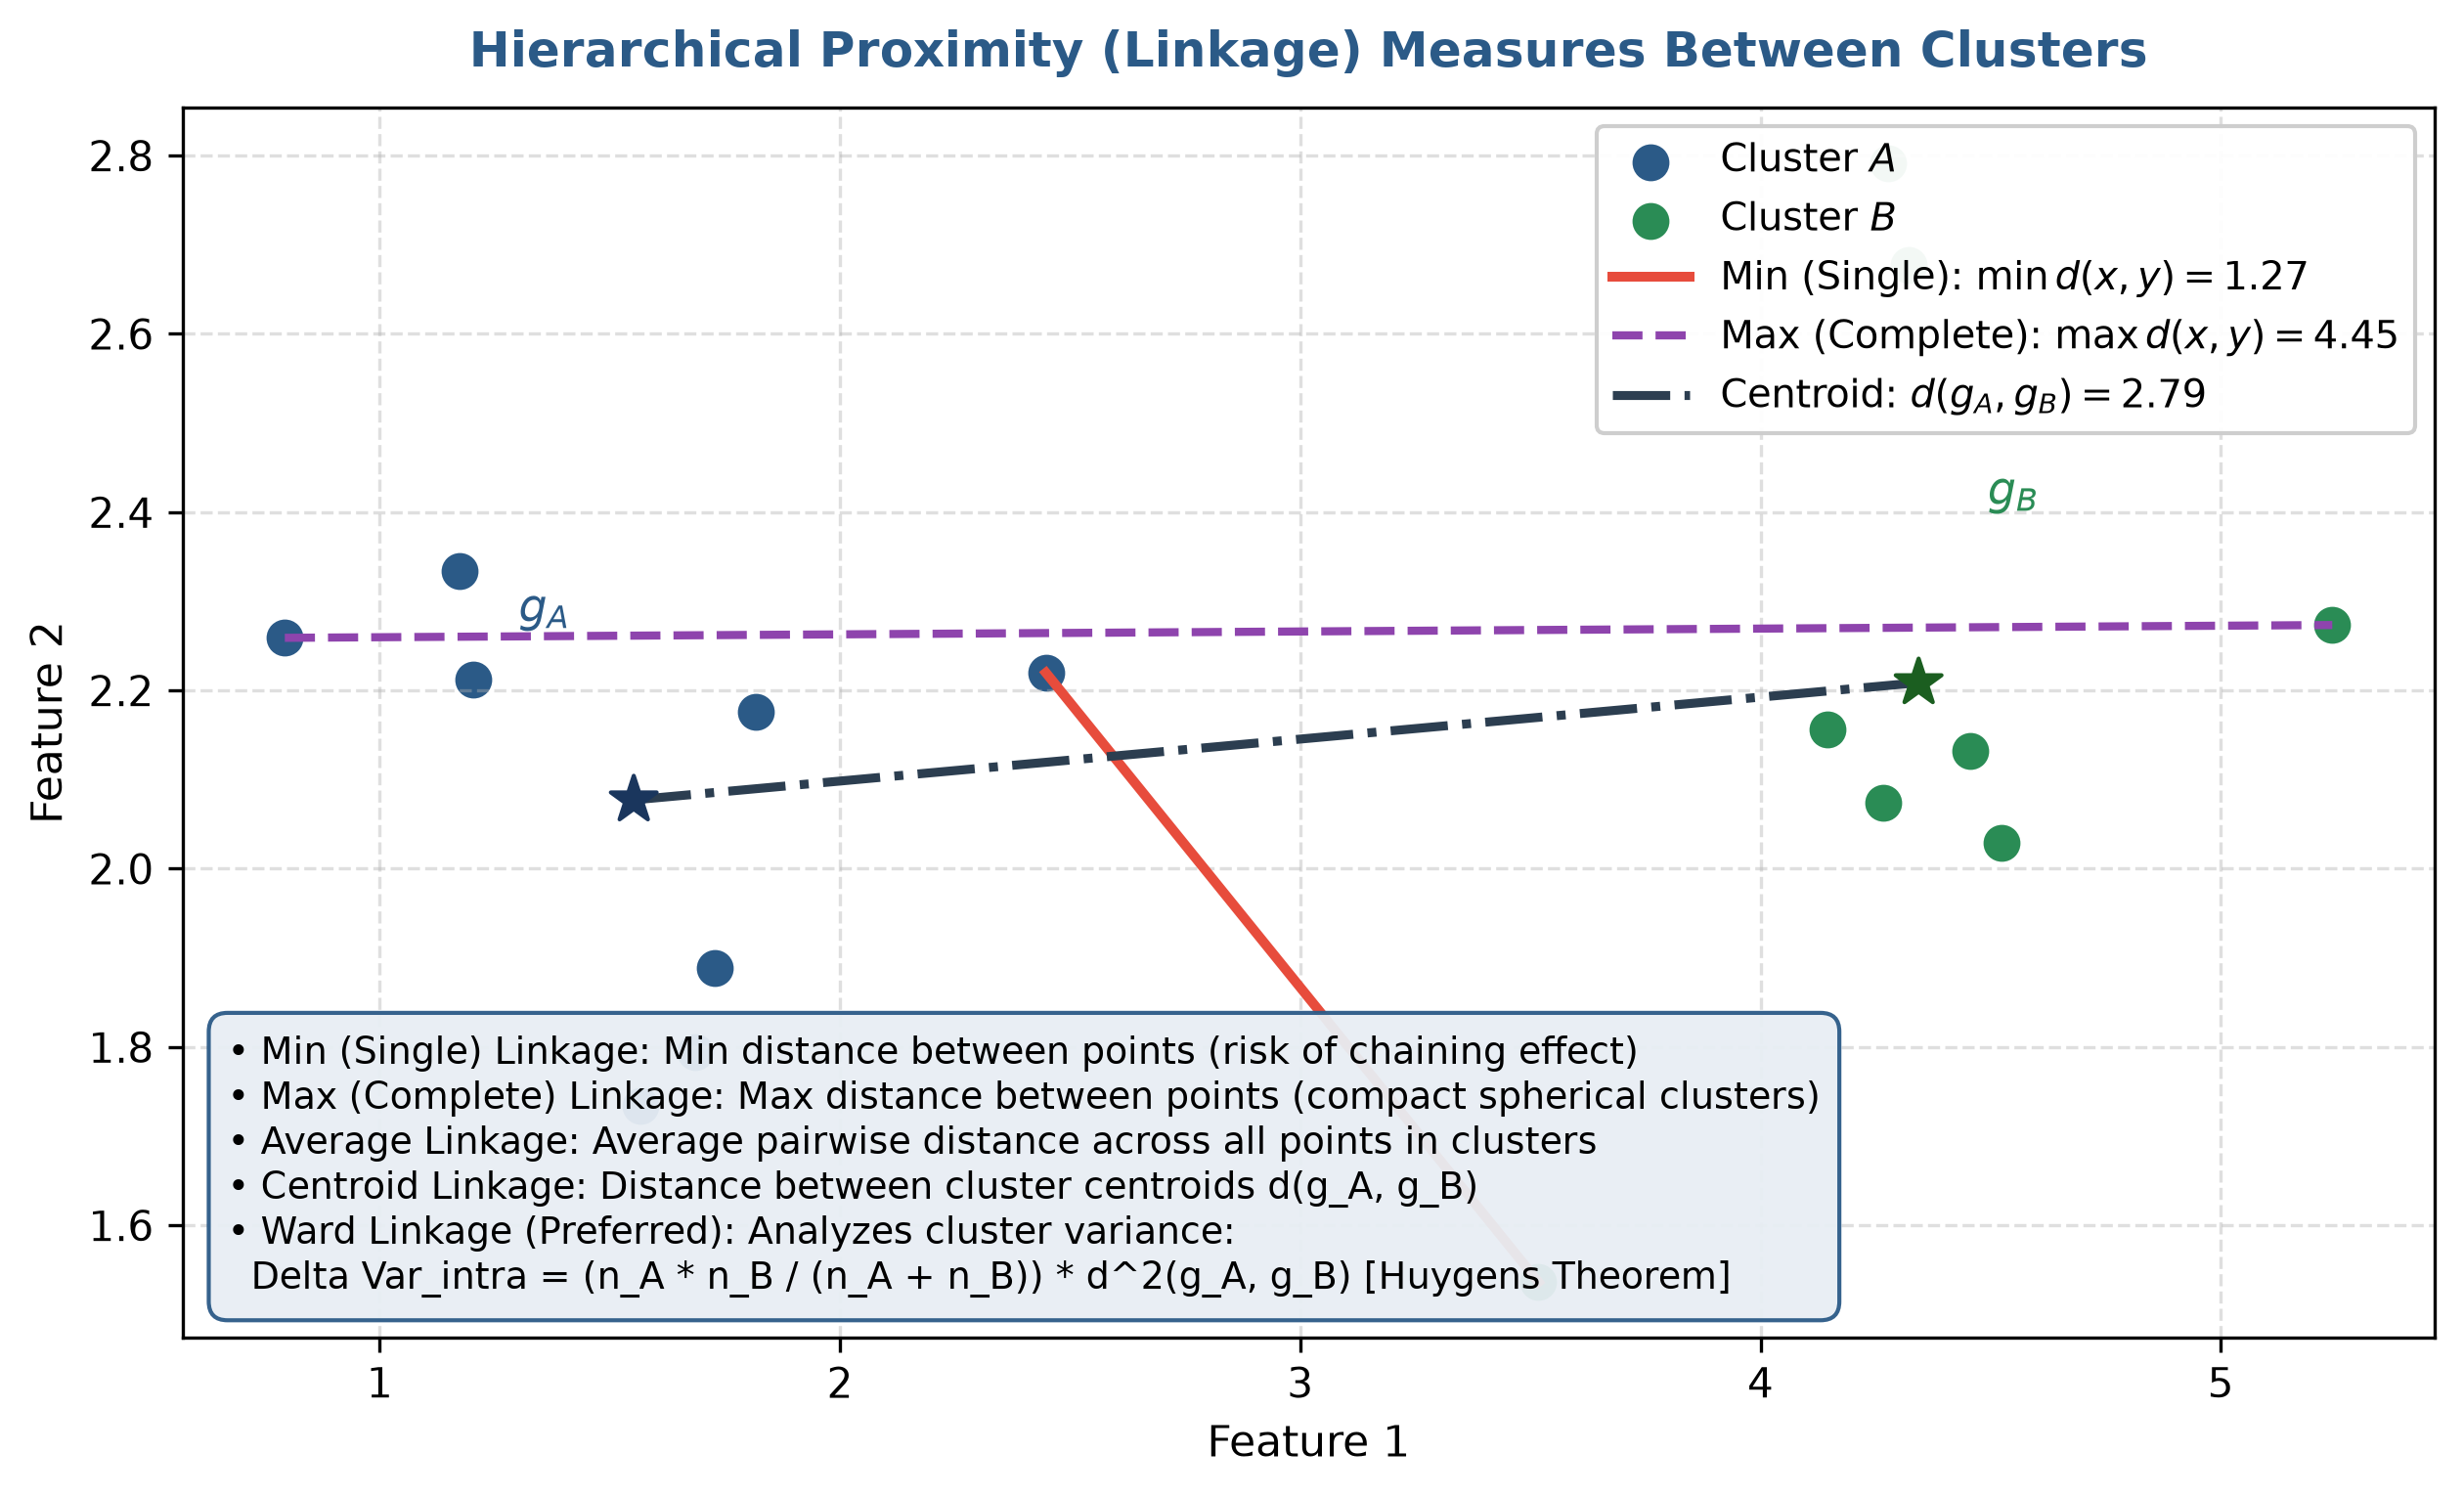
\includegraphics[width=0.74\textwidth]{linkage_criteria.png}\par
\vspace{1pt}
{\footnotesize\textit{Comparison of Linkage Criteria: Min, Max, Centroid, Average, and Ward (Variance-based via Huygens).}}\par
}
\vspace{3pt}

\noindent{\large\bfseries\color{themeblue} 4.4 Properties of Hierarchical Clustering}\par\vspace{2pt}
\begin{itemize}[leftmargin=12pt, itemsep=1.5pt, topsep=1pt, parsep=0pt]
    \item Unlike K-means, hierarchical classification \textbf{does not require choosing a number of clusters beforehand}.
    \item \textbf{Deterministic:} Algorithm is \textbf{independent of the order of insertion of points}.
    \item \textbf{Complexity:} $O(n^3)$ (or $O(n^2)$ optimized).
\end{itemize}

\clearpage

% =========================================================================
% PAGE 5: Section 5: Worked Toy Example & Section 6: Comparison Table
% =========================================================================

\noindent{\Large\bfseries\color{themeblue} 5. Worked Toy Example: K-Means Iteration \& Ward Linkage}\par\vspace{3pt}
\textbf{Setup:} 4 individuals in 2D space:
$v_1 = (1, 1)$, $v_2 = (2, 1)$, $v_3 = (4, 3)$, $v_4 = (5, 4)$.\\
Global dataset centroid: $g = \frac{1}{4} \big((1,1) + (2,1) + (4,3) + (5,4)\big) = (3.0, \, 2.25)$.\\
Initial K-Means centers ($k=2$): $g_1^{(0)} = (1, 1)$, $g_2^{(0)} = (5, 4)$.

\begin{enumerate}[leftmargin=14pt, itemsep=2.5pt, topsep=1.5pt, parsep=0pt]
    \item \textbf{One K-Means Iteration (Assignment \& Centroid Update):}
    \begin{itemize}[leftmargin=10pt, itemsep=1pt]
        \item $d^2(v_1, g_1)=0 < 25 \implies v_1 \in C_1$; \quad $d^2(v_2, g_1)=1 < 18 \implies v_2 \in C_1$;
        \item $d^2(v_3, g_1)=13 > 2 \implies v_3 \in C_2$; \quad $d^2(v_4, g_1)=25 > 0 \implies v_4 \in C_2$.
        \item Partitions: $C_1 = \{v_1, v_2\}$ ($n_1 = 2$), $C_2 = \{v_3, v_4\}$ ($n_2 = 2$).
        \item Recompute centers:
        \[
        g_1^{(1)} = \frac{(1,1)+(2,1)}{2} = (1.5, \, 1.0), \qquad g_2^{(1)} = \frac{(4,3)+(5,4)}{2} = (4.5, \, 3.5)
        \]
    \end{itemize}

    \item \textbf{Variance Computation \& Huygens Verification:}
    \begin{itemize}[leftmargin=10pt, itemsep=1pt]
        \item \textbf{Intra-Cluster Variance:}
        \[
        \operatorname{Var}_{\text{intra}} = \frac{1}{4}\big( (1-1.5)^2 + (2-1.5)^2 + (4-4.5)^2 + (3-3.5)^2 + (5-4.5)^2 + (4-3.5)^2 \big) = \frac{0.25 + 0.25 + 0.5 + 0.5}{4} = \mathbf{0.375}
        \]
        \item \textbf{Inter-Cluster Variance:}
        \[
        \operatorname{Var}_{\text{inter}} = \frac{2}{4}\|(1.5, 1.0) - (3.0, 2.25)\|^2 + \frac{2}{4}\|(4.5, 3.5) - (3.0, 2.25)\|^2 = \frac{1}{2}(3.8125) + \frac{1}{2}(3.8125) = \mathbf{3.8125}
        \]
        \item \textbf{Total Variance Check:} $\operatorname{Var}_{\text{total}} = 0.375 + 3.8125 = \mathbf{4.1875}$.\\
        Direct check: $\frac{1}{4}\sum_{i=1}^4 \|v_i - g\|^2 = \frac{5.5625 + 2.5625 + 1.5625 + 7.0625}{4} = \mathbf{4.1875}$ (identical!).
    \end{itemize}

    \item \textbf{Ward Linkage Merge Cost:}
    If clusters $C_1$ and $C_2$ were to be merged in hierarchical clustering using Ward's method:
    \[
    \Delta \operatorname{Var}_{\text{intra}}(C_1, C_2) = \frac{n_1 n_2}{n_1 + n_2} d^2(g_1, g_2) = \frac{2 \times 2}{2 + 2} \big( (1.5 - 4.5)^2 + (1.0 - 3.5)^2 \big) = 1 \cdot (9 + 6.25) = \mathbf{15.25}
    \]
\end{enumerate}

\vspace{4pt}

\noindent{\Large\bfseries\color{themeblue} 6. Comparison: K-Means vs. Hierarchical Clustering}\par\vspace{3pt}
\begin{center}
\small
\begin{tabular}{p{0.28\textwidth}p{0.32\textwidth}p{0.32\textwidth}}
\toprule
\rowcolor{lightbg}
\textbf{Property} & \textbf{K-Means (Partitioning)} & \textbf{Hierarchical Clustering} \\
\midrule
\textbf{Number of clusters $k$} & Must be specified beforehand & Not needed beforehand (cut dendrogram at chosen level) \\
\addlinespace[2pt]
\textbf{Determinism} & Sensitive to initial seeds (non-deterministic) & \textbf{Independent of insertion order} (deterministic) \\
\addlinespace[2pt]
\textbf{Output format} & Flat partition around moving centers & Hierarchical tree (\textbf{dendrogram}) \\
\addlinespace[2pt]
\textbf{Computational complexity} & \textbf{$O(N)$} (linear in data size) & \textbf{$O(n^3)$} (higher computational cost) \\
\addlinespace[2pt]
\textbf{Large dataset behavior} & Scales efficiently & Bottom of tree unreadable $\implies$ focus on top part \\
\addlinespace[2pt]
\textbf{Variance optimization} & Assigns to nearest center & \textbf{Ward linkage} (minimizes $\Delta\operatorname{Var}_{\text{intra}}$, Huygens) \\
\bottomrule
\end{tabular}
\end{center}

\end{document}
